\documentclass[12pt]{article}
\author{David Alves}

\usepackage{amsfonts}
\usepackage{amsmath}
\usepackage{amsthm}
\usepackage{dirtytalk}
\usepackage[a4paper]{geometry}
\usepackage{forest}
\usepackage{listings}
\usepackage{mathtools}
\usepackage{multicol}
\usepackage{nth}
\usepackage{relsize}
\usepackage{skak}
\usepackage{tikz}
\usepackage{tikz-qtree}
\usepackage{titling}
\usepackage{wrapfig}
\usepackage{xcolor}

\usetikzlibrary{decorations.pathreplacing}
\usetikzlibrary{patterns}

\DeclarePairedDelimiter\ceil{\lceil}{\rceil}
\DeclarePairedDelimiter\floor{\lfloor}{\rfloor}

\def\multichoose#1#2{\ensuremath{\left(\kern-.3em\left(\genfrac{}{}{0pt}{}{#1}{#2}\right)\kern-.3em\right)}}

\newcommand{\ts}[1]{\textsuperscript{#1}}

\newcommand{\ProblemStatement}[1]{
\subsection*{Problem Statement}
#1
\subsection*{Solution}
}

% If uncommented, next line hides problem statements 
%\renewcommand{\ProblemStatement}[1]{}


\title{Math 142 Problem Set 13}
\author{David Alves}
\date{2016-12-01}

\begin{document}
\pagenumbering{gobble}

\begin{center}
\large \thetitle \\
\theauthor \\
\thedate
\end{center}

\subsection*{Sources}

    \begin{itemize}
    \item http://tex.stackexchange.com and https://www.sharelatex.com for help with \LaTeX
    \end{itemize}

\section{Patriotic Octagons}
\ProblemStatement{
Suppose you have to paint each edge of an octagon red, white, or blue. Find the
number of ways to do this, counting two painting methods the same if they can be
obtained from each other by rotation.
}
 
There are 834 ways of painting the sides of an octagon red, white, or blue that
are distinct under rotation.

\begin{proof}
Let $G = C_8$, the cyclic group of 8 elements. Let 1 denote the identity
permutation in $G$, $g$ denote rotation by 1, $g^2$ denote rotation by two, etc. 
We know that $Fix(g^k)$ is the number of colors (3) to the power of the number
of cycles in $g^k$, since each cycle must have all elements the same color. 
Below are the cycles counts for each permutation.

\subsubsection*{One Cycle}

\begin{tikzpicture}
\node at (0,0) {$g$};
\node[shape=circle] (A) at (0,1.5) {1};
\node[shape=circle] (B) at (1.06,1.06) {2};
\node[shape=circle] (C) at (1.5,0) {3};
\node[shape=circle] (D) at (1.06,-1.06) {4};
\node[shape=circle] (E) at (0,-1.5) {5};
\node[shape=circle] (F) at (-1.06,-1.06) {6};
\node[shape=circle] (G) at (-1.5,0) {7};
\node[shape=circle] (H) at (-1.06,1.06) {8};
\draw [->] (A) edge[bend left=10] (B);
\draw [->] (B) edge[bend left=10] (C);
\draw [->] (C) edge[bend left=10] (D);
\draw [->] (D) edge[bend left=10] (E);
\draw [->] (E) edge[bend left=10] (F);
\draw [->] (F) edge[bend left=10] (G);
\draw [->] (G) edge[bend left=10] (H);
\draw [->] (H) edge[bend left=10] (A);
\end{tikzpicture}
\begin{tikzpicture}
\node at (0,0) {$g^7$};
\node[shape=circle] (A) at (0,1.5) {1};
\node[shape=circle] (B) at (1.06,1.06) {2};
\node[shape=circle] (C) at (1.5,0) {3};
\node[shape=circle] (D) at (1.06,-1.06) {4};
\node[shape=circle] (E) at (0,-1.5) {5};
\node[shape=circle] (F) at (-1.06,-1.06) {6};
\node[shape=circle] (G) at (-1.5,0) {7};
\node[shape=circle] (H) at (-1.06,1.06) {8};
\draw [->] (A) edge[bend right=10] (H);
\draw [->] (B) edge[bend right=10] (A);
\draw [->] (C) edge[bend right=10] (B);
\draw [->] (D) edge[bend right=10] (C);
\draw [->] (E) edge[bend right=10] (D);
\draw [->] (F) edge[bend right=10] (E);
\draw [->] (G) edge[bend right=10] (F);
\draw [->] (H) edge[bend right=10] (G);
\end{tikzpicture}
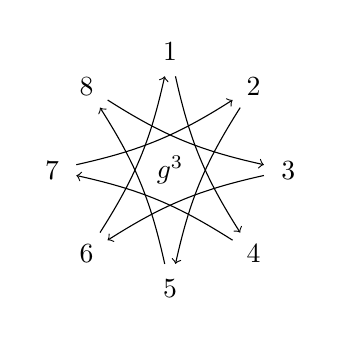
\begin{tikzpicture}
\node at (0,0) {$g^3$};
\node[shape=circle] (A) at (0,1.5) {1};
\node[shape=circle] (B) at (1.06,1.06) {2};
\node[shape=circle] (C) at (1.5,0) {3};
\node[shape=circle] (D) at (1.06,-1.06) {4};
\node[shape=circle] (E) at (0,-1.5) {5};
\node[shape=circle] (F) at (-1.06,-1.06) {6};
\node[shape=circle] (G) at (-1.5,0) {7};
\node[shape=circle] (H) at (-1.06,1.06) {8};
\draw [->] (A) edge[bend right=10] (D);
\draw [->] (B) edge[bend right=10] (E);
\draw [->] (C) edge[bend right=10] (F);
\draw [->] (D) edge[bend right=10] (G);
\draw [->] (E) edge[bend right=10] (H);
\draw [->] (F) edge[bend right=10] (A);
\draw [->] (G) edge[bend right=10] (B);
\draw [->] (H) edge[bend right=10] (C);
\end{tikzpicture}
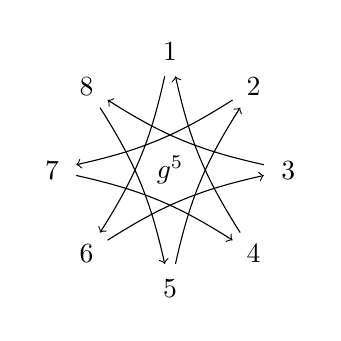
\begin{tikzpicture}
\node at (0,0) {$g^5$};
\node[shape=circle] (A) at (0,1.5) {1};
\node[shape=circle] (B) at (1.06,1.06) {2};
\node[shape=circle] (C) at (1.5,0) {3};
\node[shape=circle] (D) at (1.06,-1.06) {4};
\node[shape=circle] (E) at (0,-1.5) {5};
\node[shape=circle] (F) at (-1.06,-1.06) {6};
\node[shape=circle] (G) at (-1.5,0) {7};
\node[shape=circle] (H) at (-1.06,1.06) {8};
\draw [->] (A) edge[bend left=10] (F);
\draw [->] (B) edge[bend left=10] (G);
\draw [->] (C) edge[bend left=10] (H);
\draw [->] (D) edge[bend left=10] (A);
\draw [->] (E) edge[bend left=10] (B);
\draw [->] (F) edge[bend left=10] (C);
\draw [->] (G) edge[bend left=10] (D);
\draw [->] (H) edge[bend left=10] (E);
\end{tikzpicture}

\subsubsection*{Two Cycles}
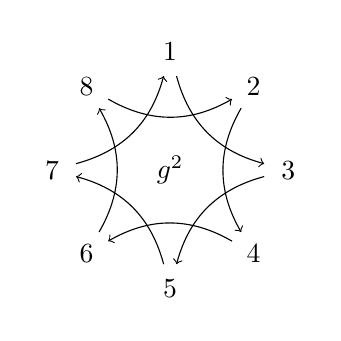
\begin{tikzpicture}
\node at (0,0) {$g^2$};
\node[shape=circle] (A) at (0,1.5) {1};
\node[shape=circle] (B) at (1.06,1.06) {2};
\node[shape=circle] (C) at (1.5,0) {3};
\node[shape=circle] (D) at (1.06,-1.06) {4};
\node[shape=circle] (E) at (0,-1.5) {5};
\node[shape=circle] (F) at (-1.06,-1.06) {6};
\node[shape=circle] (G) at (-1.5,0) {7};
\node[shape=circle] (H) at (-1.06,1.06) {8};
\draw [->] (A) edge[bend right=30] (C);
\draw [->] (B) edge[bend right=30] (D);
\draw [->] (C) edge[bend right=30] (E);
\draw [->] (D) edge[bend right=30] (F);
\draw [->] (E) edge[bend right=30] (G);
\draw [->] (F) edge[bend right=30] (H);
\draw [->] (G) edge[bend right=30] (A);
\draw [->] (H) edge[bend right=30] (B);
\end{tikzpicture}
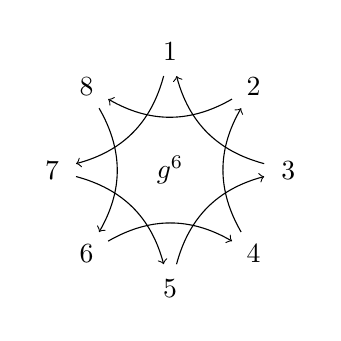
\begin{tikzpicture}
\node at (0,0) {$g^6$};
\node[shape=circle] (A) at (0,1.5) {1};
\node[shape=circle] (B) at (1.06,1.06) {2};
\node[shape=circle] (C) at (1.5,0) {3};
\node[shape=circle] (D) at (1.06,-1.06) {4};
\node[shape=circle] (E) at (0,-1.5) {5};
\node[shape=circle] (F) at (-1.06,-1.06) {6};
\node[shape=circle] (G) at (-1.5,0) {7};
\node[shape=circle] (H) at (-1.06,1.06) {8};
\draw [->] (A) edge[bend left=30] (G);
\draw [->] (B) edge[bend left=30] (H);
\draw [->] (C) edge[bend left=30] (A);
\draw [->] (D) edge[bend left=30] (B);
\draw [->] (E) edge[bend left=30] (C);
\draw [->] (F) edge[bend left=30] (D);
\draw [->] (G) edge[bend left=30] (E);
\draw [->] (H) edge[bend left=30] (F);
\end{tikzpicture}\\


\noindent\begin{minipage}{.35\textwidth}
\subsubsection*{Four Cycles}
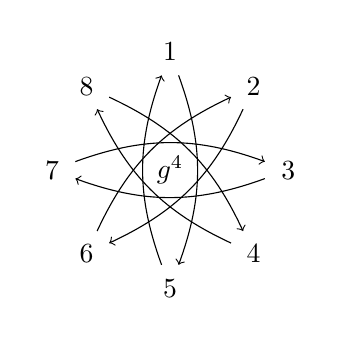
\begin{tikzpicture}
\node at (0,0) {$g^4$};
\node[shape=circle] (A) at (0,1.5) {1};
\node[shape=circle] (B) at (1.06,1.06) {2};
\node[shape=circle] (C) at (1.5,0) {3};
\node[shape=circle] (D) at (1.06,-1.06) {4};
\node[shape=circle] (E) at (0,-1.5) {5};
\node[shape=circle] (F) at (-1.06,-1.06) {6};
\node[shape=circle] (G) at (-1.5,0) {7};
\node[shape=circle] (H) at (-1.06,1.06) {8};
\draw [->] (A) edge[bend left=20] (E);
\draw [->] (B) edge[bend left=20] (F);
\draw [->] (C) edge[bend left=20] (G);
\draw [->] (D) edge[bend left=20] (H);
\draw [->] (E) edge[bend left=20] (A);
\draw [->] (F) edge[bend left=20] (B);
\draw [->] (G) edge[bend left=20] (C);
\draw [->] (H) edge[bend left=20] (D);
\end{tikzpicture}
\end{minipage}%
\begin{minipage}{.5\textwidth}
\subsubsection*{Eight Cycles}
\begin{tikzpicture}
\node at (0,.15) {\textbf{(id)}};
\node[shape=circle] (A) at (0,1.5) {1};
\node[shape=circle] (B) at (1.06,1.06) {2};
\node[shape=circle] (C) at (1.5,0) {3};
\node[shape=circle] (D) at (1.06,-1.06) {4};
\node[shape=circle] (E) at (0,-1.5) {5};
\node[shape=circle] (F) at (-1.06,-1.06) {6};
\node[shape=circle] (G) at (-1.5,0) {7};
\node[shape=circle] (H) at (-1.06,1.06) {8};
\draw [->] (A) edge[loop above,looseness=4] (A);
\draw [->] (B) edge[loop above,looseness=4] (B);
\draw [->] (C) edge[loop above,looseness=4] (C);
\draw [->] (D) edge[loop above,looseness=4] (D);
\draw [->] (E) edge[loop above,looseness=4] (E);
\draw [->] (F) edge[loop above,looseness=4] (F);
\draw [->] (G) edge[loop above,looseness=4] (G);
\draw [->] (H) edge[loop above,looseness=4] (H);
\end{tikzpicture}
\end{minipage}

Therefore we have the following cardinalities for $Fix(g^k)$:

\begin{center}
\begin{tabular}{ rcccl }
    $|Fix(1)|  $ &=& $3^8$ &=& 6561\\
    $|Fix(g)|  $ &=& $3^1$ &=& 3\\
    $|Fix(g^2)|$ &=& $3^2$ &=& 9\\
    $|Fix(g^3)|$ &=& $3^1$ &=& 3\\
    $|Fix(g^4)|$ &=& $3^4$ &=& 81\\
    $|Fix(g^5)|$ &=& $3^1$ &=& 3\\
    $|Fix(g^6)|$ &=& $3^2$ &=& 9\\
    $|Fix(g^7)|$ &=& $3^1$ &=& 3\\
\end{tabular}
\end{center}

By the Polya-Burnside theorem, the number of orbits (aka distinct paintings
after considering rotation) is $\frac{1}{|G|}\sum_{g \in G} |Fix(g)|$, thus we
have $\frac{1}{8}(6561 + 3 + 9 + 3 + 81 + 3 + 9 + 1) = $ 834 total ways to
paint the octagon.
\end{proof}


\section{Thanksgiving Dinner}
\ProblemStatement{
Your grandmother cooked a turkey, stuffng, cornbread, 2 distinguishable salads
(Caesar and spinach) and 3 distinguishable desserts (pumpkin pie, chocolate
mayhem cake, and sweet potato pie). You're allowed to eat or not eat any
particular of these 8 dishes (we assume you have infinite stomach space), but
you have to follow The Granny's Rule, which is that you cannot have any type of
dessert if you do not eat at least one salad. How many ways of eating are there?
(again, we do not care about the amount you are eating of each food, just
whether you eat it or not).  
}

There are 200 possible ways of eating.

\begin{proof}
Assume for a moment that only the 2 salads and 3 deserts existed. There would be 4
possibilities for salad consumption and 8 possibilities for dessert consumption.
3 of the 4 salad possibilities (the ones where at least one salad is eaten)
allow any dessert possibility, while the last one (where no salad is eaten)
allows only one desert possibility (the one where no desert is eaten). Thus we
have $3 \times 8 + 1 \times 1 = 25$ possible meals when we only consider salad
and desert. There are no restrictions on the other courses, so for each of those
25 valid salad-dessert combinations there are 8 possibilities for the
other dishes, giving $8 \times 25 = 200$ possible meals in total.
\end{proof}


\section{Thankfulness}
\ProblemStatement{
What are you thankful for?
}

I'm thankful for my health and my family. It's been a good year and we've been
very fortunate. In particular my wife and I had a baby daughter in January and
she's happy and healthy, so I'm very thankful for her.

\section{Generating with Powers of Ten}
\ProblemStatement{
Show with generating functions that every nonnegative integer has a unique
decimal expansion (think about what this means; consult earlier homework for
help).
}

\begin{proof}
We can represent the decimal expansions using this generating function:

\[
\prod_{i=0}^{\infty} \left(1 + x^{10^i} + x^{2\times10^i} + \dots + x^{8\times10^i} + x^{9\times10^i}\right)
\]

The term where $i=0$ is the ones place, $i=1$ is the tens place, etc., while the 10 choices inside the parentheses represent the choices for that digit. In order to show that every nonnegative integer has a unique representation, we must show that 

\[
\prod_{i=0}^{\infty} \left(1 + x^{10^i} + x^{2\times10^i} + \dots + x^{8\times10^i} + x^{9\times10^i}\right) = 1 + x + x^2 + x^3 + \dots
\]

We prove this by induction. Let $p(n)$ be the following statement:

\[
\prod_{i=0}^{n} \left(1 + x^{10^i} + x^{2\times10^i} + \dots + x^{8\times10^i} + x^{9\times10^i}\right) = 1 + x + x^2 + x^3 + \dots + x^{10^{n+1}-1}
\]
\\
$p(0)$ is the statement $(1 + x + x^2 + x^3 + \dots + x^8 + x^9) = (1 + x + x^2 + x^3+ \dots + x^8 + x^9)$, which is true. Next we must show that if $p(n)$ is true, $p(n+1)$ must also be true.\\


Multiplying both sides of $p(n)$ by $(1 + x^{10^{n+1}} + x^{2\times10^{n+1}} + \dots + x^{8\times10^{n+1}} + x^{9\times10^{n+1}})$ gives:

\begin{align*}
\prod_{i=0}^{n+1} \left(1 + x^{10^i} + x^{2\times10^i} + \dots + x^{8\times10^i} + x^{9\times10^i}\right) = 
                    (1)\left(1 + x + x^2 + x^3 + \dots + x^{10^{n+1}-1}\right) + \\
\left(x^{       {10^{n+1}}}\right)\left(1 + x + x^2 + x^3 + \dots + x^{10^{n+1}-1}\right) +\\
\left(x^{2\times{10^{n+1}}}\right)\left(1 + x + x^2 + x^3 + \dots + x^{10^{n+1}-1}\right) +\\
\left(x^{3\times{10^{n+1}}}\right)\left(1 + x + x^2 + x^3 + \dots + x^{10^{n+1}-1}\right) +\\
\left(x^{4\times{10^{n+1}}}\right)\left(1 + x + x^2 + x^3 + \dots + x^{10^{n+1}-1}\right) +\\
\left(x^{5\times{10^{n+1}}}\right)\left(1 + x + x^2 + x^3 + \dots + x^{10^{n+1}-1}\right) +\\
\left(x^{6\times{10^{n+1}}}\right)\left(1 + x + x^2 + x^3 + \dots + x^{10^{n+1}-1}\right) +\\
\left(x^{7\times{10^{n+1}}}\right)\left(1 + x + x^2 + x^3 + \dots + x^{10^{n+1}-1}\right) +\\
\left(x^{8\times{10^{n+1}}}\right)\left(1 + x + x^2 + x^3 + \dots + x^{10^{n+1}-1}\right) +\\
\left(x^{9\times{10^{n+1}}}\right)\left(1 + x + x^2 + x^3 + \dots + x^{10^{n+1}-1}\right) +\\
\end{align*}
Multiplying through gives 
\begin{align*}
\prod_{i=0}^{n+1} \left(1 + x^{10^i} + x^{2\times10^i} + \dots + x^{8\times10^i} + x^{9\times10^i}\right) = 
\left(1 + x + x^2 + \dots + x^{10^{n+1}-2} + x^{10^{n+1}-1}\right) + \\
\left(x^{10^{n+1}} + x^{10^{n+1}+1} + x^{10^{n+1}+2} + \dots + x^{10^{n+1} + x^{10^{n+1}-2}} + x^{10^{n+1} + x^{10^{n+1}-1}}\right) +\\
\left(x^{2\times10^{n+1}} + x^{2\times10^{n+1}+1} + x^{2\times10^{n+1}+2} + \dots + x^{2\times10^{n+1} + 10^{n+1}-2} + x^{2\times10^{n+1} + 10^{n+1}-1}\right) +\\
\left(x^{3\times10^{n+1}} + x^{3\times10^{n+1}+1} + x^{3\times10^{n+1}+2} + \dots + x^{3\times10^{n+1} + 10^{n+1}-2} + x^{3\times10^{n+1} + 10^{n+1}-1}\right) +\\
\left(x^{4\times10^{n+1}} + x^{4\times10^{n+1}+1} + x^{4\times10^{n+1}+2} + \dots + x^{4\times10^{n+1} + 10^{n+1}-2} + x^{4\times10^{n+1} + 10^{n+1}-1}\right) +\\
\left(x^{5\times10^{n+1}} + x^{5\times10^{n+1}+1} + x^{5\times10^{n+1}+2} + \dots + x^{5\times10^{n+1} + 10^{n+1}-2} + x^{5\times10^{n+1} + 10^{n+1}-1}\right) +\\
\left(x^{6\times10^{n+1}} + x^{6\times10^{n+1}+1} + x^{6\times10^{n+1}+2} + \dots + x^{6\times10^{n+1} + 10^{n+1}-2} + x^{6\times10^{n+1} + 10^{n+1}-1}\right) +\\
\left(x^{7\times10^{n+1}} + x^{7\times10^{n+1}+1} + x^{7\times10^{n+1}+2} + \dots + x^{7\times10^{n+1} + 10^{n+1}-2} + x^{7\times10^{n+1} + 10^{n+1}-1}\right) +\\
\left(x^{8\times10^{n+1}} + x^{8\times10^{n+1}+1} + x^{8\times10^{n+1}+2} + \dots + x^{8\times10^{n+1} + 10^{n+1}-2} + x^{8\times10^{n+1} + 10^{n+1}-1}\right) +\\
\left(x^{9\times10^{n+1}} + x^{9\times10^{n+1}+1} + x^{9\times10^{n+1}+2} + \dots + x^{9\times10^{n+1} + 10^{n+1}-2} + x^{9\times10^{n+1} + 10^{n+1}-1}\right)\\
\end{align*}

which can be simplified to 

\[
\prod_{i=0}^{n+1} \left(1 + x^{10^i} + x^{2\times10^i} + \dots + x^{8\times10^i} + x^{9\times10^i}\right) = 1 + x + x^2 + x^3 + \dots + x^{10^{n+2}-1}
\]

Since this is $p(n+1)$, we have shown that if $p(n)$ is true then $p(n+1)$ must be true, which completes the inductive proof.


\end{proof}

\section{Majority Rules}
\ProblemStatement{
Say $(2n + 1)$ people, including you, have a majority vote in a company for
allowing or disallowing hats to be worn in the company. If you know everyone
else is going to vote uniformly randomly for \say{yes} or \say{no}, what is the
probability that your vote is \say{critical}? (we define your vote to be
\say{critical} if after we fix everyone else's vote, you voting one way or
other changes the result) (optional: with a computer, explore the probability
that your vote is critical for big $n$, or for there being 3 outcomes instead
of 2)
}

The probability that your vote is \say{critical} is 
\[
    \binom{2n}{n}\left(\frac{1}{2}\right)^{2n}
\]

\begin{proof}
First we observe that your vote is only critical if the other $2n$ votes
are tied with $n$ voting yes and $n$ voting no. If they were not tied, there
would have to be at least $n+1$ votes on one side and at most $n-1$ votes on
the other, so your vote would not be critical since there is a difference of
two. 

There are $\binom{2n}{n}$ ways to choose the $n$ yes votes from among the $2n$
total votes. For each of those ways, the probability that it will occur is
$(\frac{1}{2})^n$ (the chance that all $n$ of the yes voters will vote yes)
times $(\frac{1}{2})^n$ (the chance that all $n$ of the no voters will vote
no). This gives an overall probability of $\binom{2n}{n}(\frac{1}{2})^{2n}$
\end{proof}

\subsection*{Optional}
Here's a Python program which generates $2n$ random votes and measures how often they are evenly split for large values of $n$:
\begin{center}
\begin{lstlisting}[language=Python]
#!/usr/bin/env python3
import random

def is_close(n):
    v = random.getrandbits(2*n)
    return bin(v).count('1') == n

def p_close(n, trials):
    return sum(is_close(n) for i in range(trials)) / trials

for exp in range(20):
    n = 2**exp
    trials = min(2**24, 2**(34-exp))
    print(exp, n, trials, p_close(n, trials), sep='\t')
\end{lstlisting}
\end{center}

\noindent Here's a table summarizing the output:

\begin{center}
\begin{tabular}{ lllr }
\hline
    $n$ & Measured Probability & Predicted Probability & Trials Run\\
\hline
$2^0    = 1     $ & 0.5001128315925598    & 0.5                 & 16777216 \\
$2^1    = 2     $ & 0.37497973442077637   & 0.375               & 16777216 \\
$2^2    = 4     $ & 0.2733776569366455    & 0.273438            & 16777216 \\
$2^3    = 8     $ & 0.19642597436904907   & 0.196381            & 16777216 \\
$2^4    = 16    $ & 0.13995373249053955   & 0.13995             & 16777216 \\
$2^5    = 32    $ & 0.09931820631027222   & 0.0993468           & 16777216 \\
$2^6    = 64    $ & 0.07034200429916382   & 0.0703861           & 16777216 \\
$2^7    = 128   $ & 0.04979640245437622   & 0.0498191           & 16777216 \\
$2^8    = 256   $ & 0.03525400161743164   & 0.0352446           & 16777216 \\
$2^9    = 512   $ & 0.02493804693222046   & 0.02492780589297954 & 16777216 \\
$2^{10} = 1024  $ & 0.017606258392333984  & 0.01762877240484652 & 16777216 \\
$2^{11} = 2048  $ & 0.012477874755859375  & 0.0124661853637603  & 8388608  \\
$2^{12} = 4096  $ & 0.008898258209228516  & 0.0088151932204816  & 4194304  \\
$2^{13} = 8192  $ & 0.006194591522216797  & 0.0062333780167465  & 2097152  \\
$2^{14} = 16384 $ & 0.004390716552734375  & 0.0044076974932754  & 1048576  \\
$2^{15} = 32768 $ & 0.003177642822265625  & 0.0031167246762524  & 524288   \\
$2^{16} = 65536 $ & 0.00229644775390625   & 0.0022038613571975  & 262144   \\
$2^{17} = 131072$ & 0.00154876708984375   & 0.0015583667966430  & 131072   \\
$2^{18} = 262144$ & 0.00140380859375      & 0.001101932254924   & 65536    \\
$2^{19} = 524288$ & 0.000946044921875     & 0.000779183955637   & 32768    \\
\end{tabular}
\end{center}

\section{Time Spent \& Thoughts}

This was a much easier problem set than usual. Problem \#1 tests a hard to understand topic, but it's a very straightforward application of the topic, so it wasn't bad. The decimal problem was a huge pain just because of the volume of equations and making sure that I didn't have any typos in them. I enjoyed the optional part of problem 5, but the rest of the problem set wasn't very interesting. I spent about four hours doing this homework.

\end{document}
